\documentclass[border=8pt]{standalone}
\usepackage{fontspec}
\setsansfont{Arial}
\usepackage{pgfplots}
\pgfplotsset{compat=1.18,
  every axis/.append style={/pgf/number format/assume math mode=true,
    tick label style={font=\sffamily\small},
    nodes near coords style={font=\sffamily\scriptsize}}}
% Fixed operating point (confidence 0.25, IoU 0.50) on the published test set.
% Source: docs/t41-results.md, Results table (PR #25).
\begin{document}
\sffamily\small
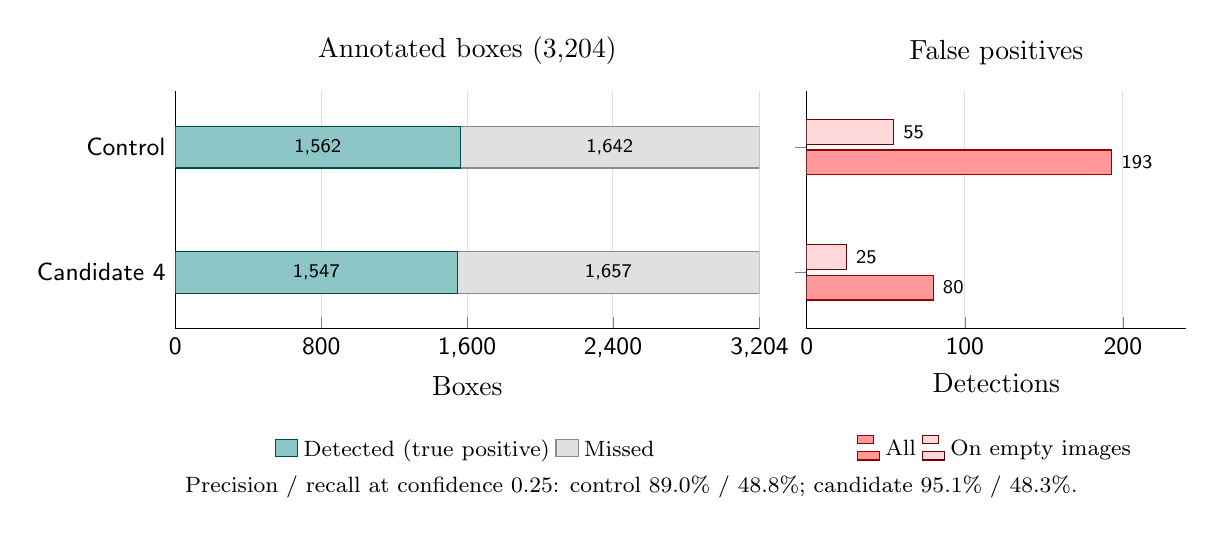
\begin{tikzpicture}
\begin{axis}[
  name=boxes,
  width=9cm,height=4.6cm,
  xbar stacked,bar width=15pt,
  xmin=0,xmax=3204,xtick={0,800,1600,2400,3204},
  symbolic y coords={Candidate 4,Control},ytick=data,
  enlarge y limits=0.45,
  title={Annotated boxes (3{,}204)},xlabel={Boxes},
  xmajorgrids,grid style={black!12},axis lines*=left,
  nodes near coords,
  legend style={font=\footnotesize,draw=none,fill=none,at={(0.5,-0.42)},anchor=north,legend columns=-1},
]
\addplot[fill=teal!45,draw=teal!60!black] coordinates {(1547,Candidate 4) (1562,Control)};
\addplot[fill=black!12,draw=black!45] coordinates {(1657,Candidate 4) (1642,Control)};
\legend{Detected (true positive),Missed}
\end{axis}
\begin{axis}[
  at={(boxes.east)},anchor=west,xshift=0.6cm,
  width=6.4cm,height=4.6cm,
  xbar,bar width=9pt,
  xmin=0,xmax=240,
  symbolic y coords={Candidate 4,Control},ytick=data,yticklabels={},
  enlarge y limits=0.45,
  title={False positives},xlabel={Detections},
  xmajorgrids,grid style={black!12},axis lines*=left,
  nodes near coords,
  legend style={font=\footnotesize,draw=none,fill=none,at={(0.5,-0.42)},anchor=north,legend columns=-1},
]
\addplot[fill=red!40,draw=red!60!black] coordinates {(80,Candidate 4) (193,Control)};
\addplot[fill=red!15,draw=red!45!black] coordinates {(25,Candidate 4) (55,Control)};
\legend{All,On empty images}
\end{axis}
\node[font=\footnotesize,anchor=north west] at ([yshift=-1.75cm]boxes.south west)
  {Precision / recall at confidence 0.25: control 89.0\% / 48.8\%; candidate 95.1\% / 48.3\%.};
\end{tikzpicture}
\end{document}
